\begin{lstlisting}[language=Python, caption={Qiskit code}, label={lst:qiskit-circuit}]
import qiskit
from qiskit import QuantumCircuit, transpile
from qiskit_aer import AerSimulator
from qiskit.visualization import plot_histogram
import matplotlib.pyplot as plt
from qiskit.qasm3 import dumps

# step 0: create a Quantum Circuit
qc = QuantumCircuit(2, 2)  # 2 qubits, 2 classical bits

# step 1:
qc.h(0)
qc.h(1)

# step 2:
qc.cz(1, 0)

# step 3:
qc.h(0)
qc.h(1)

# step 4:
qc.x(0)
qc.x(1)

# step 5:
qc.cz(1, 0)

# step 6:
qc.x(0)
qc.x(1)

# step 7:
qc.h(0)
qc.h(1)

# measure q[0] -> c[0]; measure q[1] -> c[1];
qc.measure(0, 0)
qc.measure(1, 1)

qc.draw('mpl')  # draw circuit diagram
\end{lstlisting}





\begin{figure}[H]
    \centering
    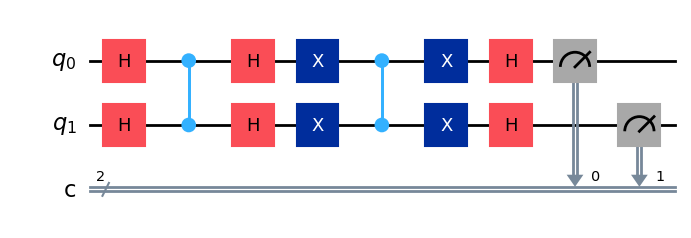
\includegraphics[width=0.7\textwidth]{images/circuit.png}
    \caption{Qiskit circuit}
    \label{fig:qiskit circuit}
\end{figure}

\begin{lstlisting}[language=Python, caption={Histogram with zero-count states}, label={lst:qiskit-hist}]
%matplotlib inline
from qiskit.visualization import plot_histogram

try:
    n_bits = len(next(iter(counts)))
except StopIteration:
    n_bits = getattr(qc, "num_qubits", 2)

labels = [format(i, f"0{n_bits}b") for i in range(2**n_bits)]
complete_counts = {b: counts.get(b, 0) for b in labels}

fig = plot_histogram(complete_counts, title="Measurements", bar_labels=True)
fig.show()
\end{lstlisting}



\begin{figure}[H]
    \centering
    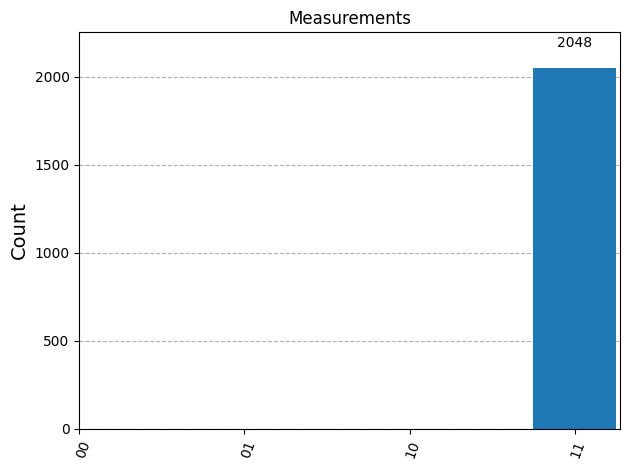
\includegraphics[width=0.7\textwidth]{images/histograms.png}
    \caption{output histogram}
    \label{fig:output histogram}
\end{figure}

%% Qasm 
\begin{lstlisting}[language=Python, caption={Export circuit to QASM3}, label={lst:qasm-export}]
qasm_str = dumps(qc)
print(qasm_str)
\end{lstlisting}

\begin{lstlisting}[language=Python, caption={Output generato: OpenQASM 3}, label={lst:qasm3-output}, backgroundcolor=\color{bg}]
OPENQASM 3.0;
include "stdgates.inc";
bit[2] c;
qubit[2] q;
h q[0];
h q[1];
cz q[1], q[0];
h q[0];
h q[1];
x q[0];
x q[1];
cz q[1], q[0];
x q[0];
x q[1];
h q[0];
h q[1];
c[0] = measure q[0];
c[1] = measure q[1];
\end{lstlisting}





